\documentclass[11pt, a4paper]{article}

\usepackage{graphicx}
\usepackage[a4paper,top=3cm,bottom=2cm,left=2cm,right=2cm,marginparwidth=1.75cm]{geometry}
\usepackage[english]{babel}
\usepackage[utf8x]{inputenc}
\usepackage{subfig}
\usepackage{float}
\usepackage{amsmath}
\usepackage{amssymb}
\usepackage{mhchem}
\usepackage{hyperref}
\usepackage{tikz}
\usepackage{cancel}
\usepackage{bm}

\graphicspath{ {./images} }
\newcommand*{\qed}{\hfill\ensuremath{\quad\square}}%
\newcommand*{\rad}{\ensuremath{\,\text{rad}}}
\newcommand*{\R}{\ensuremath{\mathbb{R}}}
\newcommand*{\C}{\ensuremath{\mathbb{C}}}
\renewcommand*{\Re}{\operatorname{Re}}
\renewcommand*{\Im}{\operatorname{Im}}
\renewcommand*{\epsilon}{\varepsilon}
\renewcommand*{\phi}{\varphi}
\renewcommand*{\d}{\text{d}}

\DeclareRobustCommand{\uvec}[1]{{%
  \ifcat\relax\noexpand#1%
    % it should be a Greek letter
    \bm{\hat{#1}}%
  \else
    \ifcsname uvec#1\endcsname
      \csname uvec#1\endcsname
    \else
      \bm{\hat{\mathbf{#1}}}%
     \fi
   \fi
}}

\makeatletter
\renewcommand*\env@matrix[1][*\c@MaxMatrixCols c]{%
  \hskip -\arraycolsep
  \let\@ifnextchar\new@ifnextchar
  \array{#1}}
\makeatother

\newtheorem{theorem}{Theorem}
\numberwithin{equation}{section}
\numberwithin{figure}{section}

%------------------------------------------------
%Templates for images and figures
% \begin{figure}[h]
%   \centering
%   \subfloat[caption 1]{{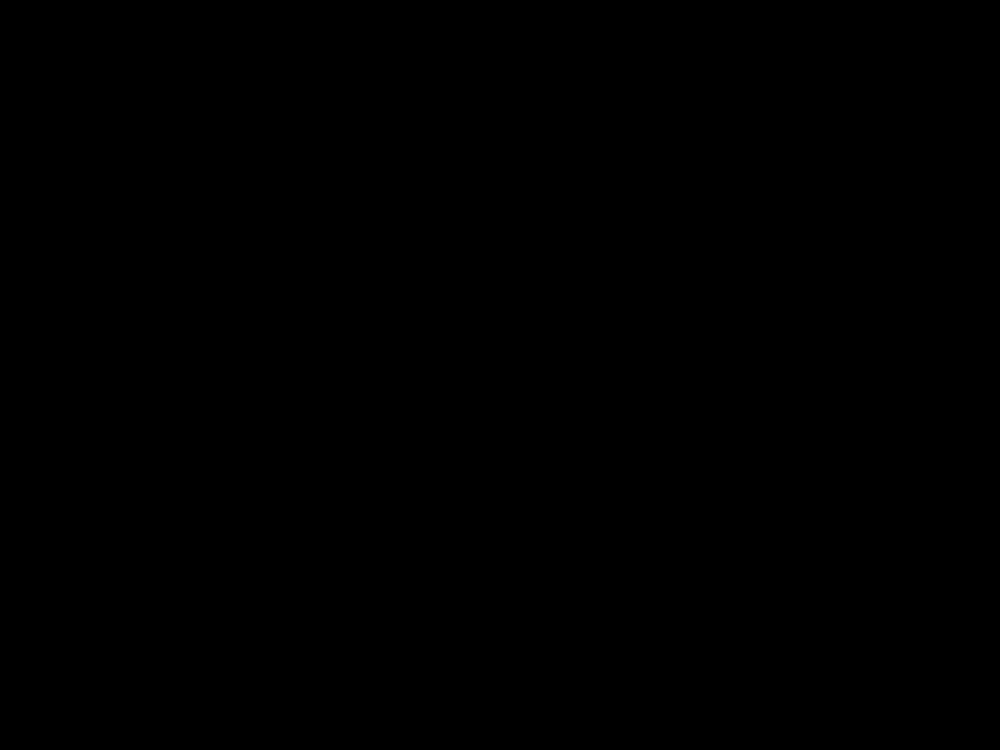
\includegraphics[width=30mm]{images/placeholder.png}}}%
%   \qquad
%   \subfloat[caption 2]{{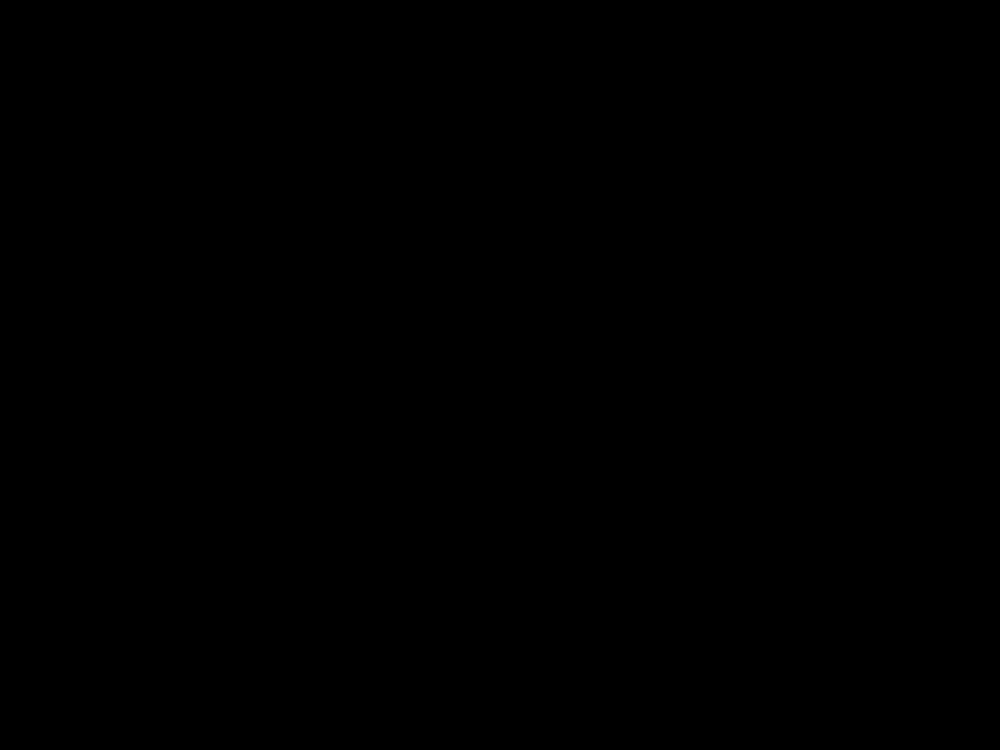
\includegraphics[width=30mm]{images/placeholder.png}}}%
%   \caption{Description}
% \end{figure}

% \begin{figure}[h]
%   \centerline{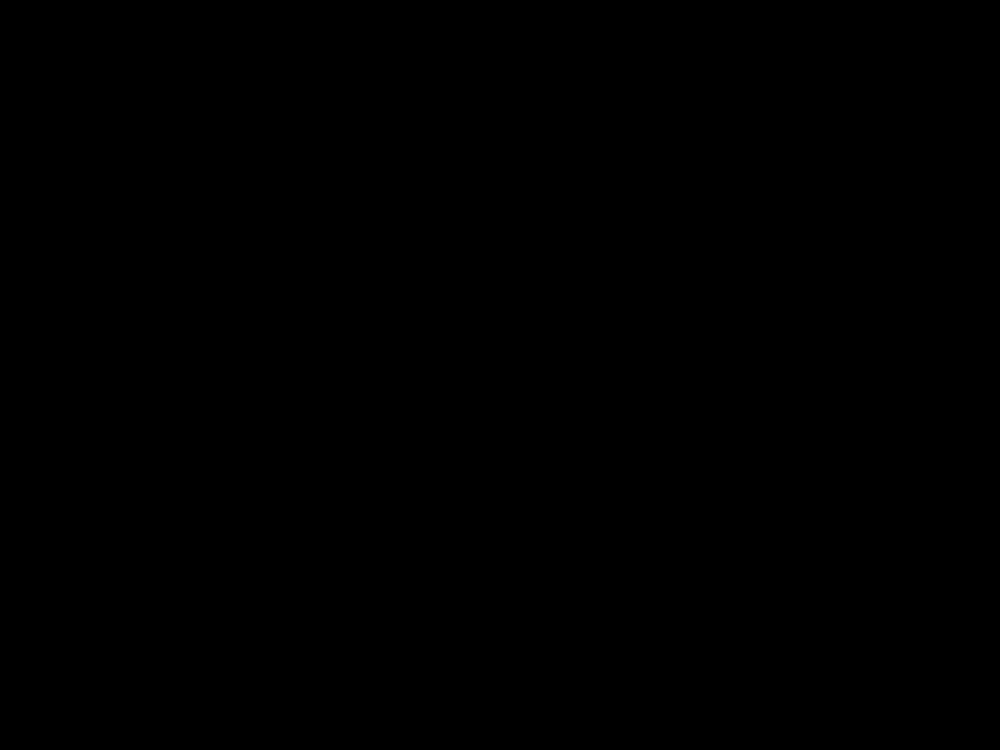
\includegraphics[width=50mm]{images/placeholder.png}}
%   \caption{Description}
% \end{figure}

%Template for a simple table 
%\begin{table}[h]
%   \caption{Description} %title of the table
%   \centering % centering table
%   \begin{tabular}{l rr} % creating three columns
%     \hline\hline %inserting double-line
%     & & \\ [0.5ex] % Insert half line vertical spacing
%     \hline % inserts single-line
%     & & \\ 
%     & & \\
%     & & \\
%     & & \\
%   \hline % inserts single-line
%   \end{tabular}
%   \label{tab:hresult}
% \end{table}
%-----------------------------------------------

\begin{document}
\setcounter{section}{5}
\section{Describing rotation using Euler angles}

\subsection{Euler angles and rotation matrices}
Rather then describing rotation in terms of angles between unit vectors in triads we can also specify 3 angles for rotation to fully describe orientation. In the case of Euler angle we describe rotation using the yaw-pitch-roll convention. Yaw describes rotation about the $Z$ axis of the $\mathcal{N}$ tiad by an angle of $\psi$ where $\psi\in[0, 2\pi)$. We create an intermediate triad $\mathcal{F}$ after the yaw rotation with the axis $x'$, $y'$ and $z'$. Pitch happens about the $y'$ axis of this intermediate triad by an angle of $\theta$, where $\theta\in[0, 2\pi)$. This creates another intermediate triad that we call $\mathcal{G}$ with the axis $x''$, $y''$ and $z''$. Finally we roll about the $x''$ axis of this second intermediate triad by an angle of $\phi$ where $\phi\in\left[-\frac{\pi}{2}, \frac{\pi}{2}\right]$. This creates our final triad $\mathcal{B}$. We can describe these 3 succesive rotations in terms of matrices. Since the rotation only happens about one axis at a time we can simplify the rotation matrix which gives the following:
\begin{align}
  ^\mathcal{B}C_\mathcal{N} &= \,^\mathcal{B}C_\mathcal{G}(\phi)\,^\mathcal{G}C_\mathcal{F}(\theta)\,^\mathcal{F}C_\mathcal{N}(\psi)\\
  &= 
  \begin{bmatrix}
    1 & 0 & 0\\
    0 & \cos(\phi) & \sin(\phi)\\
    0 & -\sin(\phi) & \cos(\phi)\\
  \end{bmatrix}
  \begin{bmatrix}
    \cos(\theta) & 0 & \sin(\theta)\\
    0 & 1 & 0\\    
    -\sin(\theta) & 0 & \cos(\theta)\\
  \end{bmatrix}
  \begin{bmatrix}
    \cos(\psi) & \sin(\psi) & 0\\
    -\sin(\psi) & \cos(\psi) & 0\\
    0 & 0 & 1\\
  \end{bmatrix}
\end{align}


\subsection{Principal action of rotation}
Euler's rotation theorem states that every chain of 3 succesive rotation can also be described by a single rotation about the principal axis of rotation. This principal axis of rotation implies that there exists a subspace which under the transformation of the rotation matrix stays the same and unscaled. From this we can conclude 2 things:
\begin{enumerate}
  \item The rotation matrix has an eigenvalue of 1
  \item The eigenvector corresponding to this eigenvalue is the direction for the principal axis of rotation.
\end{enumerate}


\end{document}